
%%%%%%%%%%%%%%%%%%%%%%%%%%%%%%%%%%%%%%%%%%%%%%%%%%%%%%%%
%
% Copyright (c) 2003-2010 by University of Queensland
% Earth Systems Science Computational Center (ESSCC)
% http://www.uq.edu.au/esscc
%
% Primary Business: Queensland, Australia
% Licensed under the Open Software License version 3.0
% http://www.opensource.org/licenses/osl-3.0.php
%
%%%%%%%%%%%%%%%%%%%%%%%%%%%%%%%%%%%%%%%%%%%%%%%%%%%%%%%%


\section{Some Remarks on Lumping}
\label{REMARKS ON LUMPING}

When using explicit time integration schemes (we will discuss two examples later in this section)
very small time steps need to be used in order to maintain stability. In orer to reduce 
computational costs at each time step lumping of the coefficient matrix to a diagonal matrix
is appled reducing costs for updating the solution to a simple component-by-component 
vector-vector product. Although lumping can speed-up simulations dramatically
it needs to be applied with some care. In this section we will briefly discuss
two commonly used techiques, namely row sum lumping 
\index{linear solver!row sum lumping}\index{row sum lumping} and HRZ 
lumping \index{linear solver!HRZ lumping}\index{HRZ lumping}.

As an example for an hyperpolic problem we take a look 
at the scalar wave equation
\begin{eqnarray} \label{LUMPING WAVE} 
u_{,tt}=c^2 u_{,ii} \; .
\end{eqnarray}
The schemes are tested against the reference solution
\begin{eqnarray} \label{LUMPING WAVE TEST} 
u=sin(5 \pi (x_0-c*t) )
\end{eqnarray}
over the 2D unit square. Note that $u_{,i}n_i=0$ on faces $x_1=0$ and $x_1=1$.
On faces $x_0=0$ and $x_0=1$ the solution is constraints.

The solution scheme is explicit Verlet scheme\index{Verlet scheme} with constant time step size $dt$ given by 
\begin{eqnarray} \label{LUMPING WAVE VALET}
u^{(n)}=2u^{(n-1)}-u^{(n-2)} + dt^2 a^{(n)} \\
\end{eqnarray}
for all $n=2,3,\ldots$ where the upper index ${(n)}$ refers to values at time $t^{(n)}=t^{(n-1)}+h$ and
$a^{(n)}$ is the solution of 
\begin{eqnarray} \label{LUMPING WAVE VALET 2} 
a^{(n)}=c^2 u^{(n-1)}_{,ii} \; .
\end{eqnarray}
The equation is read as a PDE for the unknown $a^{(n)}$ which needs to be solved in each time-step. 
In the notation of equation~\ref{LINEARPDE.SINGLE.1} we need to set $D=1$ and 
$X=-c^2 u^{(n-1)}_{,i}$. In order to maintain stability the time step size needs to fullfill 
Courant–Friedrichs–Lewy condition (CFL condition)\index{Courant condition}\index{explicit scheme!Courant condition} which 
in the case discussed here takes the form
\begin{eqnarray} \label{LUMPING WAVE CFL} 
dt = f \cdot \frac{dx}{c} .
\end{eqnarray}
where $dx$ is the mesh size and $f$ is a safty factor. Here we use $f=\frac{1}{6}$.

\begin{figure}
\centerline{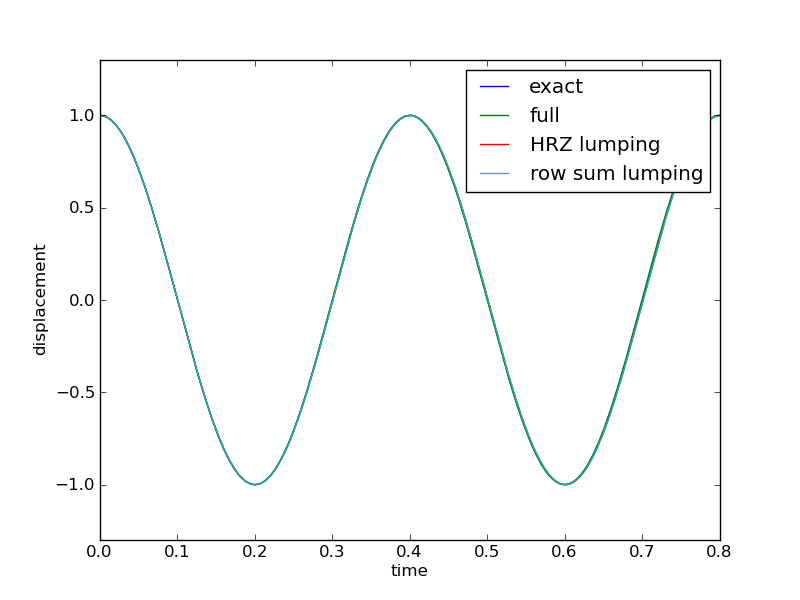
\includegraphics[width=7cm]{lumping_valet_a_1}}
\caption{Amplitude at point $(\frac{1}{2},\frac{1}{2})$ using the accelaraton formulation~\ref{LUMPING WAVE VALET 2} of the 
Velet scheme with order $1$ elements, element size $dx=0.01$, and $c=1$.}
\label{FIG LUMPING VALET A}
\end{figure}

\begin{figure}
\centerline{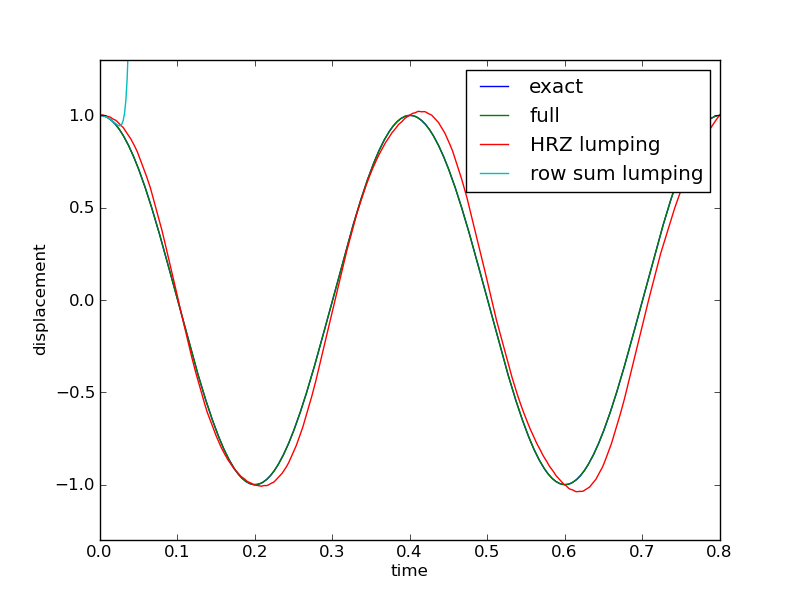
\includegraphics[width=7cm]{lumping_valet_a_2}}
\caption{Amplitude at point $(\frac{1}{2},\frac{1}{2})$ using the accelaraton formulation~\ref{LUMPING WAVE VALET 2} of the 
Velet scheme with order $2$ elements, element size $0.01$, and $c=1$.}
\label{FIG LUMPING VALET B}
\end{figure}

\begin{figure}
\centerline{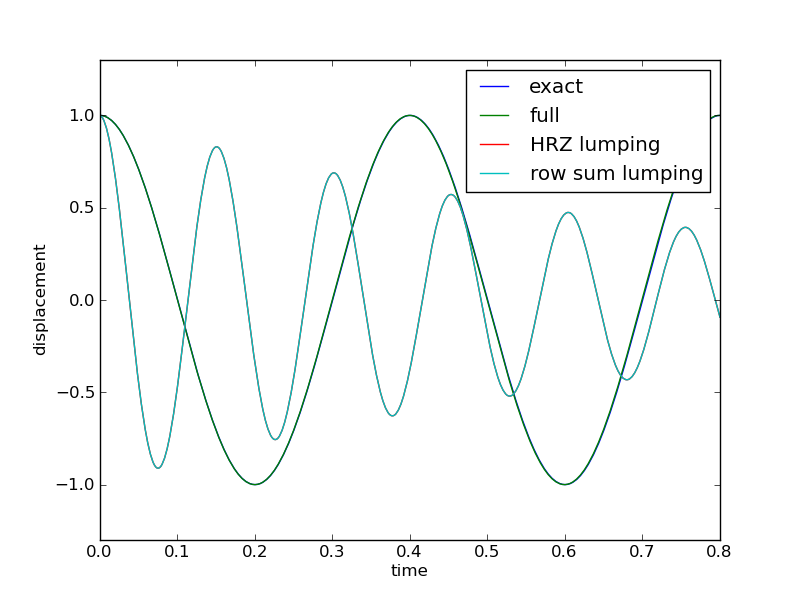
\includegraphics[width=7cm]{lumping_valet_u_1}}
\caption{Amplitude at point $(\frac{1}{2},\frac{1}{2})$ using the displacement formulation~\ref{LUMPING WAVE VALET 3} of the 
Velet scheme with order $1$ elements, element size $0.01$ and $c=1$.}
\label{FIG LUMPING VALET C}
\end{figure}

Figure~\ref{FIG LUMPING VALET A} shows a comparison between 
the exact solution, using a full mass matrix, using HRZ lumping and row sum lumping
for rectangular, order 1 elements (element size is $0.01$) at the point $(\frac{1}{2},\frac{1}{2})$
over time. All four graphs are allmost identical. As shown in
Figure~\ref{FIG LUMPING VALET B} the situation is changing when using order $2$ elements. 
In fact one can observe that the row sum lumping is unstable (Notice that for 
row sum lumping for order $2$ elements zero row sums can be produced) while using HRZ lumping 
shows similar behaviour like using using the full mass matrix with the a
slightly slower wave propagation speed.

Alternatively, one can directly solve for $u^{(n)}$ by inserting equation~(\ref{LUMPING WAVE VALET})
into equations~\ref{LUMPING WAVE VALET 2}:
\begin{eqnarray} \label{LUMPING WAVE VALET 3} 
u^{(n)}=2u^{(n-1)}-u^{(n-2)} + (dt\cdot c)^2 u^{(n-1)}_{,ii} \; .
\end{eqnarray}
Again we can read this update as a PDE for the unknown $u^{(n)}$ which needs to be solved in each time-step. 
In the notation of equation~\ref{LINEARPDE.SINGLE.1} we need to set $D=1$, $Y=2u^{(n-1)}-u^{(n-2)}$ and 
$X=-(h\cdot c)^2 u^{(n-1)}_{,i}$. Notice that for the case of using the full mass matrix 
the accelaraton formulation~\ref{LUMPING WAVE VALET 2} and displacement formulation~\ref{LUMPING WAVE VALET 3}
are identical. Figure~\ref{FIG LUMPING VALET C} shows the result for order $1$ elements (for order $2$ both 
lumping methods are not stable). The curves for the exact and the full mass matrix approximation
are almost identical while the - in this case identical - curves for row sum and 
HRZ lumping are showing faster period with a decaying amplitude.

As a second example 
we look at the advection equation
\begin{eqnarray} \label{LUMPING ADVECTIVE} 
u_{,t}=(v_i u)_i \; .
\end{eqnarray}
where $v_i$ is a given velocity field. For our simple test we set $v_i=(1,0)$ and
\begin{equation} \label{LUMPING ADVECTIVE TEST} 
u(x,t)= 
\left\{
   \begin{array}{cl}
   1 &  x_0 < t \\
   0 &  x_0 \ge t 
   \end{array}
\right.
\end{equation}
As a solution scheme we use the two-step Taylor-Galerkin scheme \index{Taylor-Galerkin scheme}
(which is in this case equivalent to SUPG\index{SUPG}):
which in the incremental formulation is given as
\begin{eqnarray} \label{LUMPING SUPG 1} 
du^{(n-\frac{1}{2})} = \frac{dt}{2} (v_i u^{(n-1)})_i \\
du^{(n)} = dt (v_i (u^{(n-1)}+du^{(n-\frac{1}{2})}) )_i \\
u^{(n)} = u^{(n)} + du^{(n)} 
\end{eqnarray}
This can be reformulated calculating $u^{(n)}$ directly:
\begin{eqnarray} \label{LUMPING SUPG 2} 
u^{(n-\frac{1}{2})} = u^{(n-1)} + \frac{dt}{2} (v_i u^{(n-1)})_i \\
u^{(n)} =  u^{(n-1)} + dt (v_i u^{(n-\frac{1}{2})} )_i 
\end{eqnarray}
Notice that one can insert the first equation into the second to calculate $u^{(n)}$ with out the intermediate step. We
will not discuss this approach has it does not very flexible when more terms (e.f. a diffusion) into the right hand side. 
Similar to the wave propagation problem the time step size needs to fullfill a 
Courant–Friedrichs–Lewy condition (CFL condition)\index{Courant condition}\index{explicit scheme!Courant condition} which 
in the case of the advection problem takes the form
\begin{eqnarray} \label{LUMPING ADVECTION CFL} 
dt = f \cdot \frac{dx}{\|v\|} .
\end{eqnarray}
where $dx$ is the mesh size and $f$ is a safty factor. Again we use $f=\frac{1}{6}$.

\begin{figure}
\centerline{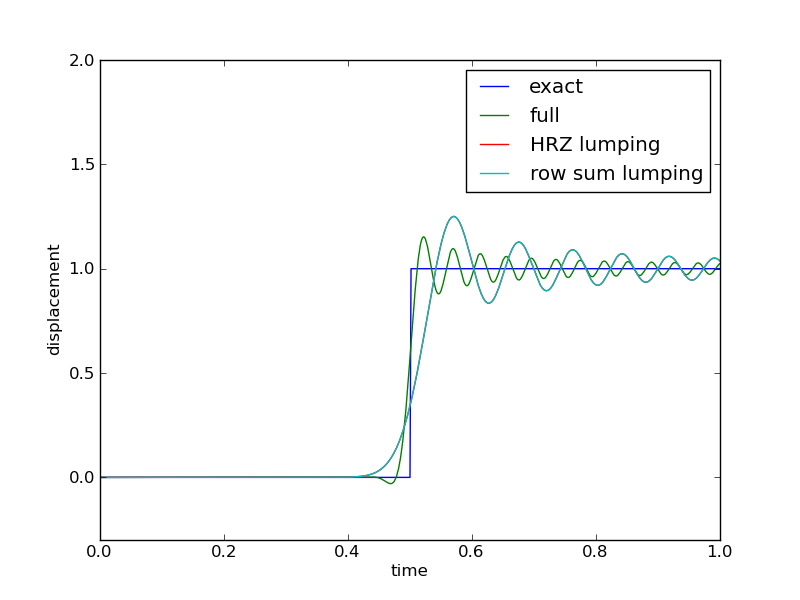
\includegraphics[width=7cm]{lumping_SUPG_du_1}}
\caption{Amplitude at point $(\frac{1}{2},\frac{1}{2})$ using the incremental formulation~\ref{LUMPING SUPG 1} of the 
Taylor-Galerkin scheme with order $1$ elements, element size $dx=0.01$, $v=(1,0)$.}
\label{FIG LUMPING SUPG INC A}
\end{figure}

\begin{figure}
\centerline{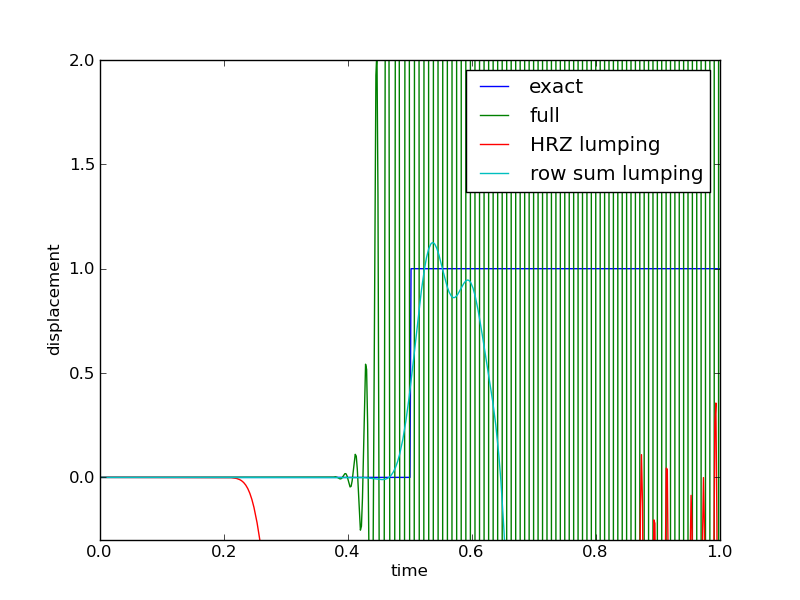
\includegraphics[width=7cm]{lumping_SUPG_du_2}}
\caption{Amplitude at point $(\frac{1}{2},\frac{1}{2})$ using the incremental formulation~\ref{LUMPING SUPG 1} of the 
Taylor-Galerkin scheme  with order $2$ elements, element size $0.01$, $v=(1,0)$.}
\label{FIG LUMPING SUPG INC B}
\end{figure}

Figures~\ref{FIG LUMPING SUPG INC A} and~\ref{FIG LUMPING SUPG INC B} show the value of the true solution,
using the exact mass matrix, the HRZ lumping and the row sum lumping for the incermental formulation. In the case of order $1$ elements
osciallation prior to the arrivial of the front and -in particular- after the front has passed. 
For order $2$ elements all techniques fail. 

\begin{figure}
\centerline{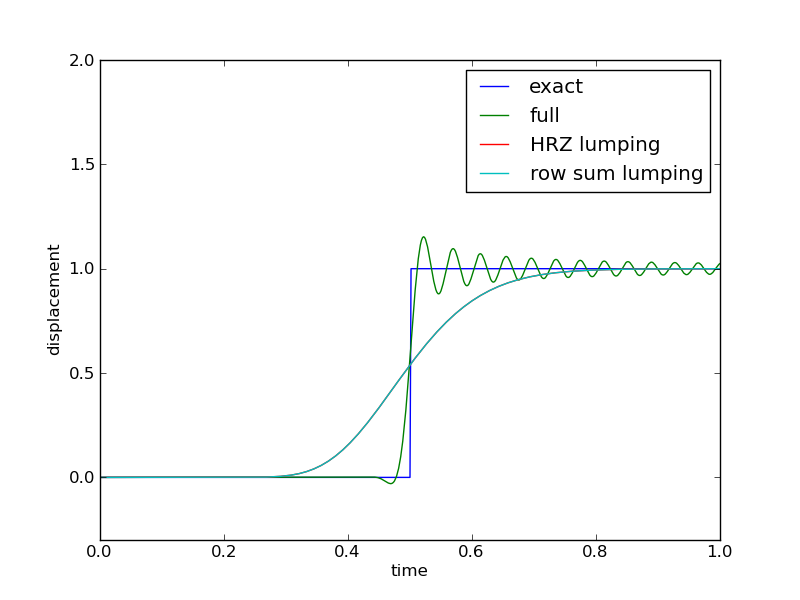
\includegraphics[width=7cm]{lumping_SUPG_u_1}}
\caption{Amplitude at point $(\frac{1}{2},\frac{1}{2})$ using the direct formulation~\ref{LUMPING SUPG 2} of the 
Taylor-Galerkin scheme using order $1$ elements, element size $dx=0.01$, $v=(1,0)$.}
\label{FIG LUMPING SUPG A}
\end{figure}
\begin{figure}
\centerline{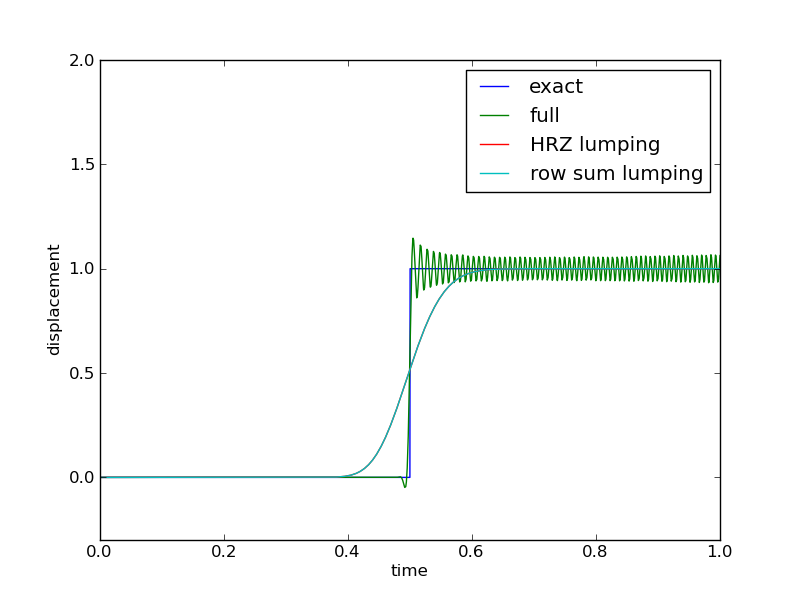
\includegraphics[width=7cm]{lumping_SUPG_u_1b}}
\caption{Amplitude at point $(\frac{1}{2},\frac{1}{2})$ using the direct formulation~\ref{LUMPING SUPG 2} of the 
Taylor-Galerkin scheme using order $1$ elements, element size $dx=0.002$, $v=(1,0)$.}
\label{FIG LUMPING SUPG Ab}
\end{figure}

\begin{figure}
\centerline{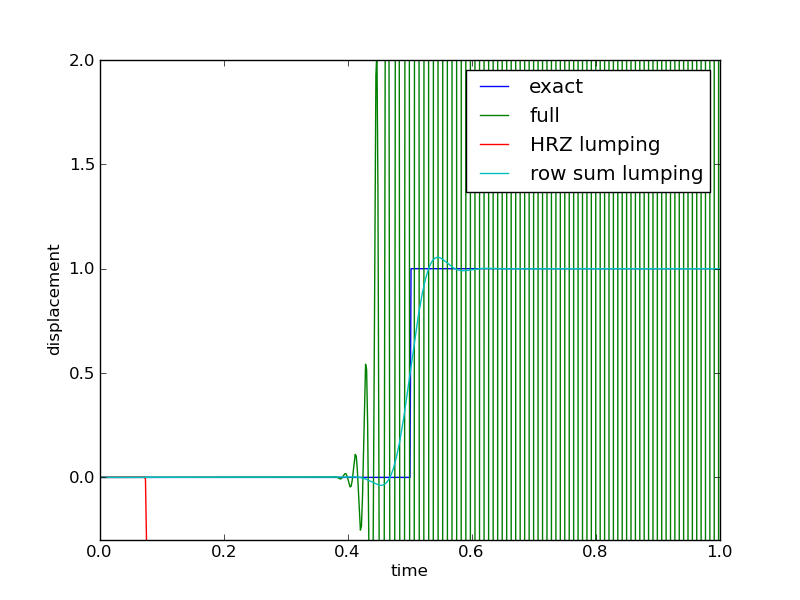
\includegraphics[width=7cm]{lumping_SUPG_u_2}}
\caption{Amplitude at point $(\frac{1}{2},\frac{1}{2})$ using the direct formulation~\ref{LUMPING SUPG 2} of the 
Taylor-Galerkin scheme  using order $2$ elements, element size $0.01$, $v=(1,0)$.}
\label{FIG LUMPING SUPG B}
\end{figure}

For the order $1$ case results are better when using the direct formulation. As shown in Figure~\ref{FIG LUMPING SUPG A}
using the full mass matrix introduces still osciallation around the time when the front hits the
observation point. Lumping (HRZ and row sum lumping are identical in our case) introduces additional 
smoothing into the solution avoiding any rippels. As confirmed by Figure~\ref{FIG LUMPING SUPG Ab}
the approximation around the time of impact improves when a smaller mesh size and lumping is used.
However, using the full mass matrix a smaller mesh size will produces stronger riples.
Figure~\ref{FIG LUMPING SUPG B} shows that
for order $2$ elements nor HRZ lumping neither using the full mass matrix is able to produce a stable solution
while row sum lumping can smooth some of the osciallations.   

In summary: For wave propagation type problem lumping produces results simular to the usage of the full mass matrix as significantly 
lower costs. An accelleration based formulation with HRZ lumping should be used which can be appied to order $1$ and order $2$
element. For transport type problems using row sum lumping is essential to achieve a smooth solution. It is not recommended to 
use second order elements.



